\section{eo\-Init$<$ EOT $>$ Class Template Reference}
\label{classeo_init}\index{eoInit@{eoInit}}
Base (name) class for Initialization of chromosomes, used in a population contructor.  


{\tt \#include $<$eo\-Init.h$>$}

Inheritance diagram for eo\-Init$<$ EOT $>$::\begin{figure}[H]
\begin{center}
\leavevmode
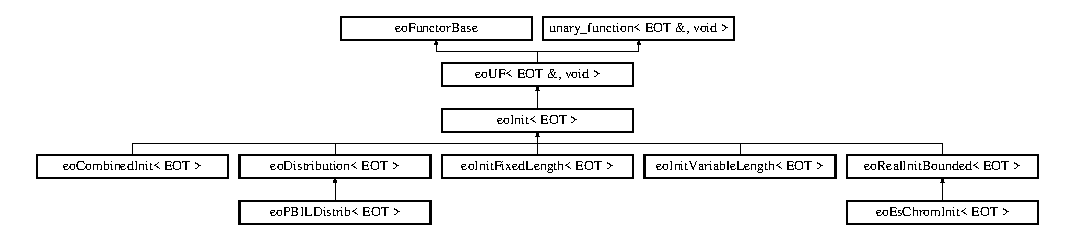
\includegraphics[height=2.78607cm]{classeo_init}
\end{center}
\end{figure}
\subsection*{Public Member Functions}
\begin{CompactItemize}
\item 
virtual std::string {\bf class\-Name} (void) const 
\begin{CompactList}\small\item\em class\-Name: Mandatory because of {\bf eo\-Combined\-Init}{\rm (p.\,\pageref{classeo_combined_init})}. \item\end{CompactList}\end{CompactItemize}


\subsection{Detailed Description}
\subsubsection*{template$<$class EOT$>$ class eo\-Init$<$ EOT $>$}

Base (name) class for Initialization of chromosomes, used in a population contructor. 

It is derived from {\bf eo\-Mon\-Op}{\rm (p.\,\pageref{classeo_mon_op})}, so it can be used inside the algorithm as well.

\begin{Desc}
\item[See also:]{\bf eo\-Pop}{\rm (p.\,\pageref{classeo_pop})} \end{Desc}




Definition at line 45 of file eo\-Init.h.

\subsection{Member Function Documentation}
\index{eoInit@{eo\-Init}!className@{className}}
\index{className@{className}!eoInit@{eo\-Init}}
\subsubsection{\setlength{\rightskip}{0pt plus 5cm}template$<$class EOT$>$ virtual std::string {\bf eo\-Init}$<$ {\bf EOT} $>$::class\-Name (void) const\hspace{0.3cm}{\tt  [inline, virtual]}}\label{classeo_init_a0}


class\-Name: Mandatory because of {\bf eo\-Combined\-Init}{\rm (p.\,\pageref{classeo_combined_init})}. 

SHould be pure virtual, but then we should go over the whole code to write the method for all derived classes ... MS 16/7/04 

Reimplemented in {\bf eo\-Combined\-Init$<$ EOT $>$} {\rm (p.\,\pageref{classeo_combined_init_a4})}, {\bf eo\-PBILDistrib$<$ EOT $>$} {\rm (p.\,\pageref{classeo_p_b_i_l_distrib_a6})}, {\bf eo\-Parse\-Tree\-Depth\-Init$<$ FType, Node $>$} {\rm (p.\,\pageref{classeo_parse_tree_depth_init_a1})}, and {\bf eo\-St\-Parse\-Tree\-Depth\-Init$<$ FType, Node $>$} {\rm (p.\,\pageref{classeo_st_parse_tree_depth_init_a1})}.

Definition at line 52 of file eo\-Init.h.

The documentation for this class was generated from the following file:\begin{CompactItemize}
\item 
eo\-Init.h\end{CompactItemize}
